\documentclass[12pt]{article}
\title{Mini Report \#1: Predicting Stock Price Movements Using Convolutional Neural Networks}
\author{Andre Sealy, Daiki Ishiyama, Swapnil Pant}
\usepackage{amsmath, amsfonts, amssymb, amsthm,}
\usepackage{tikz}
\usetikzlibrary{matrix,positioning}
\tikzset{bullet/.style={circle,fill,inner sep=2pt}}
\usepackage{braket}
\usepackage{bbold}
\usepackage[margin=1.0in]{geometry}
\usepackage{mathtools}
\usepackage{xfrac}
\usepackage{xcolor}
\newcommand{\lam}{$\lambda$}
\usepackage{pgfplots}
\tikzset{My Style/.style={samples=100, thick}}
\usepackage{graphicx}
\usepackage{pgfplots}
\usepackage{setspace}
\usepackage{enumerate}
\usepackage{hyperref}
\usepackage{array}
\usepackage{listings}
\usepackage[official]{eurosym}
\usepackage[shortlabels]{enumitem}
\usepackage{booktabs}
\usepackage{floatrow}
\usepackage{listings}
\floatsetup[table]{capposition=top}
\usepackage{appendix}
\usepackage{xcolor}
\hypersetup{
	colorlinks,
	linkcolor={red!50!black},
	citecolor={blue!50!black},
	urlcolor={blue!80!black}
}

\definecolor{codegreen}{rgb}{0,0.6,0}
\definecolor{codegray}{rgb}{0.5,0.5,0.5}
\definecolor{codepurple}{rgb}{0.58,0,0.82}
\definecolor{backcolour}{rgb}{0.95,0.95,0.92}

\lstdefinestyle{mystyle}{
	backgroundcolor=\color{backcolour},   
	commentstyle=\color{codegreen},
	keywordstyle=\color{magenta},
	numberstyle=\tiny\color{codegray},
	stringstyle=\color{codepurple},
	basicstyle=\ttfamily\footnotesize,
	breakatwhitespace=false,         
	breaklines=true,                 
	captionpos=b,                    
	keepspaces=true,                 
	numbers=left,                    
	numbersep=5pt,                  
	showspaces=false,                
	showstringspaces=false,
	showtabs=false,                  
	tabsize=2
}
\onehalfspacing

\lstset{style=mystyle}

\begin{document}
	
\maketitle

\section*{Introduction}

Trend-following strategies -- like moving averages or time-series momentum -- are widely used in practice and have been successful across many different asset classes for decades. Despite their popularity, whether or not investors can generate excess remains questionable. Many existing trend signals are heuristic-based and chosen based on intuition or empirical trial-and-error rather than a grounded, model-based approach. This motivates our question:  Can visual patterns in historical price charts predict whether a stock will rise or fall over the next 5 days?

With the rise of machine learning, there is an opportunity to learn price trends directly from data rather than imposing rigid parametric structures (like fixed-length moving averages). We examine price trends through the lens of supervised learning, treating the trend signal as something that can be trained to predict returns. We aim to bridge the gap between statistical modeling and practical trading signals. We will generate a framework that generalizes popular tend signals and allows for a data-driven optimal trend filter, which improves return predictability and economic outcomes.

\section*{Data \& Preprocessing}
\subsection*{Data Description}

For the project, we use a comprehensive dataset that employs image classification techniques to predict stock price movements, using both structured and unstructured data, totaling 54 files organized by year. The two types of files are organized by image files (.dat) and label files, which cover 27 years from 1993 to 2019. The dataset is nearly 8 GB large, with 2,061,055 individual stock samples.

\subsection*{Images}

The image files (.dat) are binary files containing 8-bit unsigned integers in grayscale format. They all have dimensions of 64x60 pixels for 20-day windows. Different dimensions exist for 5-day and 60-day windows, but they are not utilized for this project. Each image represents a visual representation of a stock's price movement and volume history. The image files in our project will represent the features of our supervised learning algorithm.

\begin{figure}[h]
	\centering
	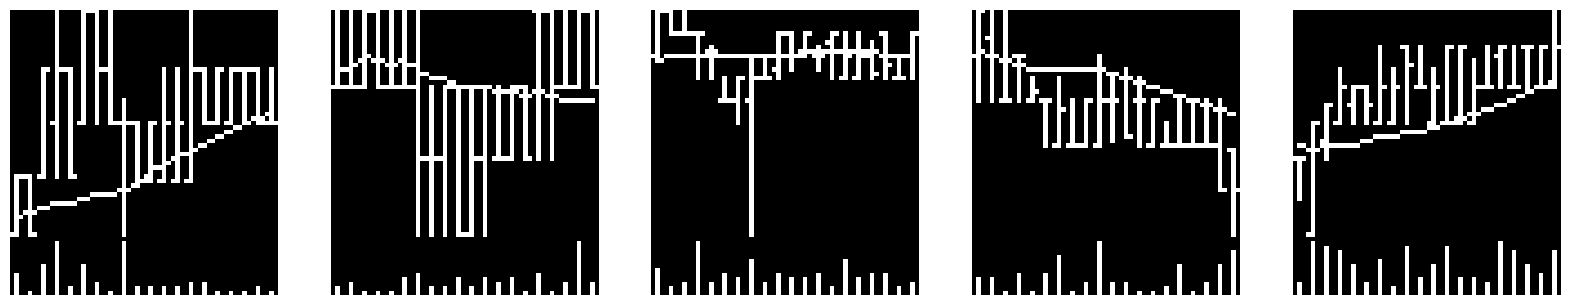
\includegraphics[width=1\linewidth]{plots/images.png}
	\caption{Generated OHLC Sample Images with Volume Bar and Moving Average Line}
	\label{fig:image}
\end{figure}

Figure (\ref{fig:image}) shows a sample of the images in our data set. Each bar on the bottom (trading volume) corresponds to the Open-High-Low-Close (OHLC) candles for a given trading day. We also see a smooth curve across the plot, which we identify as the moving average for the 20-day window.

\section*{Labels}

The labels files (.feather) represent the target variable in our dataset. Each image corresponds to a row in the matching labels file containing the following features:

\begin{itemize}
	\item Date: Last day of 20-day rolling window,
	\item StockID: CRSP PERMNO identifier,
	\item MarketCap: Market capitalization in thousands of dollars,
	\item Ret\_5d: 5-day forward return (primary prediction target),
	\item Ret\_20d: 20-day forward return,
	\item Ret\_60d: 60-day forward return,
	\item Ret\_month: Monthly return (from current month-end to next month-end),
	\item EWMA\_vol: Exponentially weighted volatility with alpha 0.05.
\end{itemize}
The classification task is to create a binary prediction of the target variable, 5-day returns (positive/negative examples), which transforms traditional time series forecasting into a visual pattern recognition problem.

\subsection*{Preprocessing}

We scale up the pipeline for multiple years, systematically loading and combining data year by year. The splitting utilized for our training and validation process involves a time-series split. We have decided to use the interval from 1993 to 2014 for our training and validation set, with the remaining 5 years for testing. This will efficiently allow our model to generalize on the unseen observations of our dataset.

Our preprocessing step also involves parallel label processing. The .feather format is specifically chosen for its performance with columnar data and fast read/write operations. After processing all of the years individually, we perform two critical concatenation operations. First, we merge all yearly image arrays into a single continuous NumPy array along the first dimension. This process creates one large tensor containing all training images. We also combine all yearly label DataFrames into a single DataFrame, preserving all column structures and maintaining alignment with the image data. The final result gives us around 1.78 million samples (1,787,748 to be exact), each with shape (64, 60) for images and 8 columns of metadata for labels.

After we perform the data aggregation step, we are left with a large NumPy array containing our image data and a DataFrame with all the corresponding labels. It should also be noted that each time we load the dataset, we create a copy of the data that detaches the data from these file mappings, preventing potential issues with file handles and memory access during training. It ensures the tensor data is contiguous in memory, which improves computational efficiency.

\subsection*{Time Series Splitting and Validation}

As mentioned previously, we use time series splitting to train the neural network, meaning we preserve the chronological ordering, which is critical for financial time series data. We take the first 70\% of samples for training and the remaining 30\% for validation. During the split, we transform the raw 5-day returns into binary labels, where label one represents the label if the 5-day return is positive and zero otherwise. This binary transformation is an important part of the preprocessing step, turning a traditional regression problem into a classification problem. (we have also created an option for random splitting but have elected not to utilize this approach)

The final part of the preprocessing involves utilizing PyTorch's DataLoader class. Using the DataLoader class, we group samples into batches of 128, which is crucial for efficient GPU processing (a form of preprocessing that transforms individual samples into structured batches). We also implement a shuffling mechanism, which randomizes the order of samples with each epoch. Randomizing the order prevents the model from learning the order of samples and reduces overfitting by presenting the data in different sequences. This process also allows us to provide more robust gradient updates.

We have also decided to implement memory pinning, which automatically pins the fetched data to CPU memory, enabling faster transfer rates to the CUDA (Compute Unified Device Architecture) enabled GPUs. This parameter also allows us to pre-allocate memory to avoid costly data transfers during training. We only use this preprocessing step for GPU-based training.

\section*{Methodology}

\subsection*{Xavier Initialization Strategy}

When working with deep neural networks, we must select an appropriate starting weight to train effectively and carefully. We accomplish this by employing the Xavier uniform initialization, which allows us to configure linear (fully connected) and convolutional layers with appropriate starting values. The Xavier initialization strategy also sets weights to values that maintain appropriate signal magnitude as data flows through the network during forward and backward propagation. By carefully scaling (and randomizing) the initialization process, we prevent the neurons from becoming saturated (outputting the same value) or becoming "dead" (never activating), which would impede the learning process, thus ensuring training stability.

The Xavier uniform initialization does this by setting the weights based on a uniform distribution with carefully calculated bounds. Afterward, we scale these initial values proportionally to each neuron's input and output connections. This process benefits networks with certain activation functions, such as ReLU. This initialization accounts for the kernel dimensions and number of filters for convolutional layers, while for linear layers, it considers the input and output dimensions.

\subsection*{Convolutional Neural Network (CNN)}

Figure (\ref{fig:cnn}) shows a visual outline of our convolutional neural network. In this section, we specifically outline the architectural components of the convolutional neural network used to train the model. The architecture processes 64x60 grayscale images representing stock price patterns and predicts binary outcomes (positive or negative future returns).

First, we describe the input layer, which reshapes to (-1, 1, 64, 60). The -1 in the first dimension allows us to take an arbitrary batch size, while the second, third, and fourth dimensions allow us to take the image's color channel, height, and width. The single grayscale channel preserves the intensity patterns of the financial charts. 

The three convolutional blocks follow the input layer. The first convolutional box has a single input channel (the greyscale) and 64 feature maps. Each convolutional block utilizes parameters for the kernel size, stride, dilation, and padding. These parameters offer the following benefits to the neural network:

\begin{itemize}
	\item \textbf{Kernel (5,3):} The kernel size fits the rectangular filter, which emphasizes the vertical patterns of the data and helps detect the short-term temporal patterns. In addition to temporal patterns, the kernel size lets us capture price formation patterns like support/resistance levels, breakouts, and trend reversals.
	\item \textbf{Stride (3,1):} The stride filter has a vertical stride of 3 and a horizontal stride of 1. This means the filter will jump 3 pixels downward after each application and move 1 pixel to the right, ensuring no pixel is skipped. This filter allows us to sample price levels more sparsely while densely sampling the dimension, which reduces the vertical dimensions of the output feature maps while preserving temporal resolution.
	\item \textbf{Dilation (2,1):} The vertical dilation (2) inserts one gap between kernel elements vertically, while the horizontal dilation (1) ensures no gaps between kernel elements, which is standard for convolutional layers. The effect of this setup expands the vertical receptive field to cover 9 pixels (5 + 4 spaces) rather than just 5. This adds the benefit of capturing broader price movements without increasing the parameter count.
	\item \textbf{Padding (12, 1):} The vertical padding adds 12 pixels of zero padding at the top and bottom, while the horizontal padding adds a minimum of 1 pixel padding at the left and right. The larger vertical padding compensates for kernel size, stride, and dilation, which allows us to ensure feature map dimensions work with subsequent layers.
\end{itemize}
After the convolutional layer, we immediately apply batch normalization, which allows us to stabilize and accelerate training by normalizing the activations between layers. The first convolutional box normalizes 64 features, while the second and third normalizes 128 and 256 features, respectively (the same number as the output channels for each convolutional layer). Batch normalization works by calculating the mean $\mu$ and variance $\sigma^2$ of activations across the batch and spatial dimensions. Then, it normalizes by applying the following transformation:
\begin{equation}
	\hat{x}=\frac{(x-\mu)}{\sqrt{\sigma^2+\epsilon}},
\end{equation}
where $\epsilon$ is some small constant used for numerical stability. We then apply a scale and shift parameter
\begin{equation}
	y=\gamma\hat{x}+\beta,
\end{equation}
where $\gamma$ is the scale and $\beta$ is the shift; which allows the network to learn the optimal distribution for each layer.

After each batch normalization process, we implement the Leaky Rectified Linear Unit (ReLU), a modified version of the standard ReLU activation function that allows a small gradient when the input is negative. This addresses the issue of vanishing gradients or "dying" layers. Each leaky ReLU will have a negative slope of 0.01. An additional benefit of using the Leaky ReLU instead of the standard ReLU is retaining some information from negative signals, which could represent important financial indicators like price drops or downtrends.

\begin{figure}[h]
	\centering
	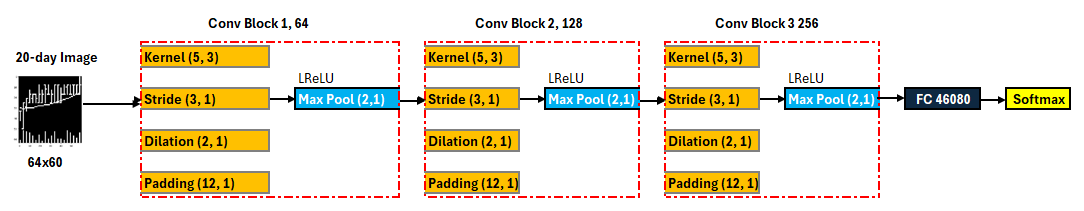
\includegraphics[width=1.05\linewidth]{plots/CNN.png}
	\caption{Visual Representation of the Convolutional Neural Network}
	\label{fig:cnn}
\end{figure}

In our CNN, we employ MaxPooling at the end of each convolutional block. MaxPooling is a downsampling operation that reduces the spatial dimensions of feature maps by selecting the maximum value within a defined window. In all three convolutional blocks, we implement the MaxPooling operation with the kernel size of (2,1) and stride of (2,1). The first implementation of MaxPooling will maintain all of the temporal information while condensing the price level, while the other two implementations will have a cumulative effect.

The final layer is a fully connected layer, which acts as a bridge from the convolutional features to the classification head of the neural network. The input dimension is 46,080, which is the direct result of flatting the output from the third convolutional block. The three convolutional blocks progressively transform the 64x60 inputs through multiple operations, while the MaxPooling operation in each block reduces the vertical dimension by half, preserving the horizontal dimension. The final output of the third block contains 256 feature maps (channels) with specific spatial dimensions, resulting in precisely 46,080 values per sample.

In this layer, we have a dropout parameter, which implements a dropout rate of 50\%. This prevents the network from over-relying on any specific feature extracted by the convolutional layer. We also use a linear projection, which directly maps the high-dimensional feature space to a binary classification. Since we have not implemented a hidden, fully connected layer, the network relies entirely on the convolutional feature hierarchy. This structure allows the convolutional layers to do the heavy lifting of feature extraction and applies a strong regularization framework at the classification stage to prevent overfitting.

For the final layer, we apply the Softmax function for the neural network, which transforms the network's raw outputs into probabilities using the following formula:

\begin{equation}
	\text{Softmax}(x_i)=\frac{e^{x_i}}{\sum_{i=1}^K e^{x_i}},
\end{equation}
where $x_i$ is the raw output (logit) for class $i$ and $K$ is the number of classes (two in relation to the objective of returns). The Softmax allows us to convert raw neural networks into probabilities between 0 and 1. It also works well with cross-entropy loss functions, providing smooth gradients for backpropagation methods and handling class imbalances in our financial data.

\subsection*{Training and Validation}

For training, we implement a complete training epoch that systematically exposes the model to all training examples, calculates prediction errors, and updates the model weights to improve performance. We process the data in batches of 128 samples (as defined by the DataLoader). The forward pass involves transferring data to the appropriate device (which will most likely be the GPU) and passing financial images through the CNN architecture. The CNN will execute the following:

\begin{itemize}
	\item Reshaping inputs to (-1, 1, 64, 60)
	\item Processing through three convolutional blocks
	\item Flattening to 46,080 features
	\item Applying dropout regularization
	\item Projecting to 2 output classes
	\item Computing final probabilities with the Softmax activation function
\end{itemize}
We implement a cross-entropy loss function to compare the predicted probabilities against the actual binary labels to quantify the prediction. For a classification of tasks with $C$ classes, the cross-entropy loss is the following:
\begin{equation}
	\text{Loss}=-\sum_{i=1}^{C}y_i\log\left(\hat{y}_i\right),
\end{equation}
where $y_i$ is the true label (one-hot encoded, so only one value is 1, and the rest are 0) and $\hat{y}_i$ is the predicted probability for class $i$ (usually from a softmax layer). In addition to the cross-entropy loss function, we implement the Adam optimizer, which adapts the learning rates for each parameter. We have set a conservative learning rate of 0.00001 to prevent overshooting optimal values.

The number of batches per epoch is determined by the size of our training dataset and the batch size defined on DataLoader. Since we are dealing with 1,787,748 samples from 1993-2014, and a 70-30 split used for training and validation, we have 1,251,424 samples. We also consider the batch size of 128. Based on these parameters, we have 9,777 batches per epoch ($1,251,424 \div 128 \approx 9,777$). Our CNN processes approximately 9,777 batches of financial images in each complete epoch. These batches allow us to provide extensive gradient updates, allowing our model to learn many patterns in the financial time series data.

For the validation process, we disable the gradient computation, which significantly reduces memory usage. This also speeds up the processing time since we're only measuring performance, not updating weights. The same cross-entropy loss function is used in the validation and training steps.

\begin{figure}[h]
	\centering
	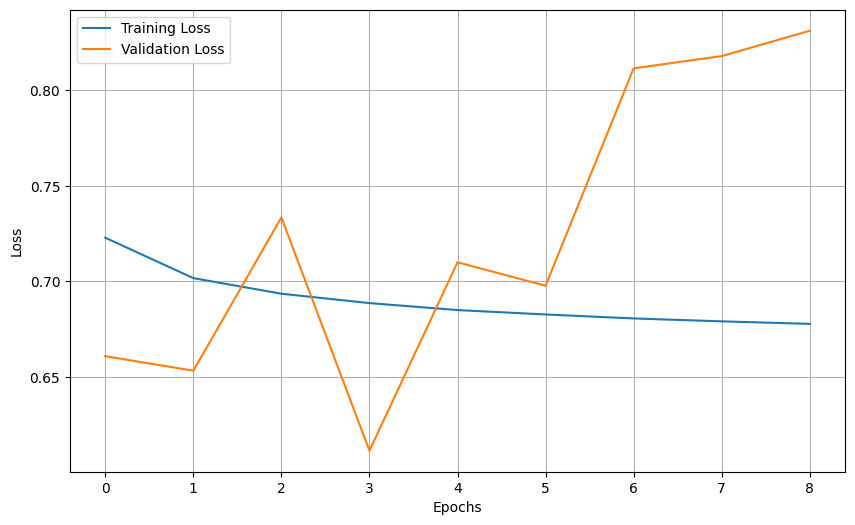
\includegraphics[width=.65\linewidth]{plots/training_validation.png}
	\caption{Training and Validation Loss}
	\label{fig:epoch_loss}
\end{figure}

We execute each epoch's training and validation process and then capture their respective loss values, our primary quantitative performance metric. The loss values directly measure how well our CNN can predict stock movements from visual chart patterns. For each epoch, we record how our financial CNN's prediction accuracy evolves, capturing both training and validation performance. We also create a system to preserve the model states throughout training, allowing us to later select optimal versions of our financial predictors based on performance metrics.

We implement an early stop logic function to determine the optimal loss characteristics. The function identifies and records when our model performs best on validation data. It identifies the best value is identified by stopping the training and validation step when the model's performance stops improving for a specific number of epochs. This prevents wasted computation time and overfitting when the model has reached its performance plateau.

Figure (\ref{fig:epoch_loss}) shows us the training and validation curves based on the epoch. Our training and validation process allowed for a maximum of 100 epochs; however, the CNN stopped after just eight epochs, suggesting that our model runs computationally efficiently with the given parameters. We look at the gap between the training and validation curve when assessing how to generalize the model. As we can see, the gap between the training and validation curves suggests that the model does not overfit, which means that we can generalize on unseen data.

For strategic functions, we save the baseline epoch on file. This allows us to resume training from this exact point if needed and provide a benchmark model for evaluation of the test data. Figure (\ref{fig:epoch_loss}) also shows us that the epoch that provides us with the best performance is epoch 3, with a training loss of 0.68597 and a validation loss of 0.611354. We have used epoch three as a benchmark for testing and evaluating the CNN.

\section*{Results}


The testing set includes the date ranges from 2015-2019, with a size of approximately 273,307 samples. Like the training and validation set, the format involves 64x60 grayscale images representing stock price patterns. Like the training and testing set, we convert continuous 5-day returns into binary classification targets (1 for positive returns, 0 for negative returns). 

We process 2,048 samples simultaneously for batch processing, significantly larger than the 128 used in the training batch size. This is possible because the testing process does not require storing gradients, which allows greater computational efficiency. Larger batches provide faster evaluation across the complete testing set of 273,307. Since we are using a time-series split, we disable any shuffling mechanism to preserve the chronological integrity of the dataset.

The question remains: Can visual patterns in historical price charts predict whether a stock will rise or fall over the next 5 days?

\subsection*{Evaluation}

\begin{figure}[h]
	\centering
	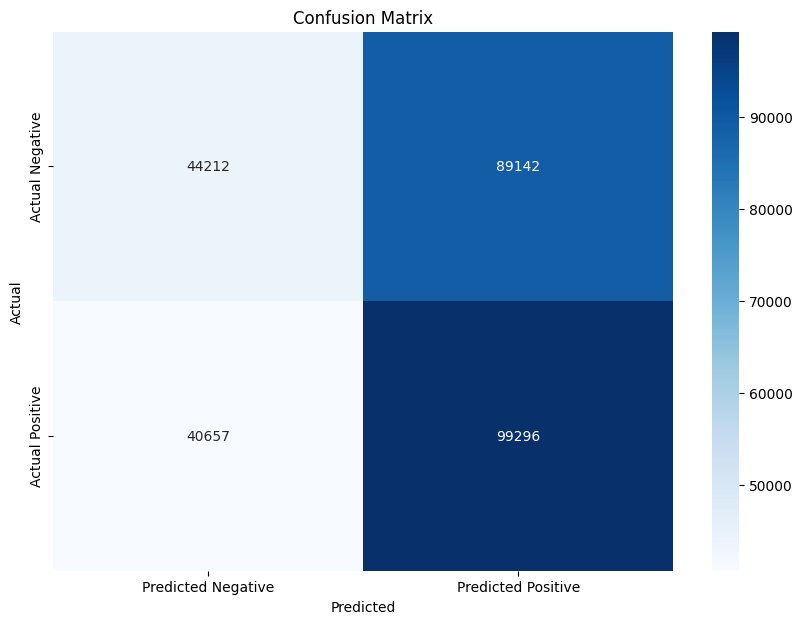
\includegraphics[width=.85\linewidth]{plots/confusion_matrix.png}
	\caption{Confusion Matrix for the Binary Classification of Returns}
	\label{fig:confusion_matrix}
\end{figure}

Similar to the training and validation step, we use the Cross-Entropy loss function for our elevation metric. The evaluation process produces three critical outputs: the test loss, the ground truth (actual market movement), and the predicted market movements. We also have the prediction probability, which we acquire through the softmax function that converts raw logits into probability distributions. With any classification function, we are only interested in the True label (index 1). The extracted probabilities represent the likelihood that each stock will experience positive returns over the next 5 days. We use the default decision threshold of 0.5.

\begin{table}[ht]
	\centering
	\caption{Metrics for the binary classification stock prediction}
	\begin{tabular}[t]{ccccc}
		\toprule
		Model & Accuracy & Precision & Recall & F1 Score \\
		\midrule
		CNN Classification & 68.95\% & 53\% & 71\% & 60\%  \\			
		\bottomrule
	\end{tabular}\label{tab:metrics}
\end{table}

Figure (\ref{fig:confusion_matrix}) shows the Confusion Matrix for the binary classification of 5d stock returns, an important visualization evaluation metric for classification models. We have stock directions predicted correctly, 143,508, with 99,296 positive correct predictions and 44,212 correct negative predictions. Along with the true positives and negatives, we have 129,799 misclassifications. From these indicators, we can predict the accuracy, which is the percentage of all predictions correctly classified, denoted by
\begin{equation}
	\text{Accuracy}=\frac{TP+TN}{(TP+TN+FP+FN)}.
\end{equation}
We also have the precision, denoted by,
\begin{equation}
	\text{Precision}=\frac{TP}{(TP+FP)};
\end{equation}
the recall, denoted by,
\begin{equation}
	\text{Recall}=\frac{TP}{(TP+FN)};
\end{equation}
and the F1 score, denoted by;
\begin{equation}
	\text{F1 Score}=\frac{2\times (\text{Precision}\times\text{Recall})}{(\text{Precision}+\text{Recall})}.
\end{equation}
Table (\ref{tab:metrics}) shows the metrics for our binary classification model using stock predictions. We use the accuracy metric to measure the overall effectiveness of our CNN, which we find to be 68.95\%. This means that our CNN is significantly better than a random guess, and more than two out of every three trades will be predicted accurately using this model. On the other hand, we must consider the precision metric, which measures the reliability of our directional signals (higher precision implies fewer false alarms when trading). We find that our precision is 53\%.

Recall indicates how many actual upward movements our model has captured. We find that 71\% of the time, our model can capture an upward trend in the stock price, which suggests fewer missed breakouts and buying opportunities. Finally, we report the F1 Score, the harmonic average of both the precision and recall metrics, which provides a balance between costly trades (false positives) and missed opportunities (false negatives). We report an F1 score of 60%.

\section*{Improvements and Future Directions}

A CNN can successfully predict stock using images from stock market prices. The predictive patterns in the pictures and labeled data provide a highly robust framework. On the other hand, this framework is not without its drawbacks. We still find issues with maintaining a higher true positive rate (53\%). However, achieving a high true positive rate may not be as important in an industry where asset prices are random. We still come away with the following questions:

\begin{itemize}
	\item Are there specific chart patterns the model struggles with?
	\item Does performance vary by market capitalization or sector?
	\item Is performance consistent across different market conditions.
\end{itemize}
For future considerations, we can lower the threshold to increase recall during uptrends when false positives are less punishing. We can also implement regime detection algorithms to automatically adjust thresholds based on current market conditions.
\end{document}